\section{Functions}
\subsection{Definition of functions}

A \textbf{function} maps elements of one set $X$ to elements of another set $Y$.
A function from $X$ to $Y$ can be viewed as a subset of $X \times Y : (x, y) \in f$ if $f$ maps $x$ to $y$.
The notation for a function is:
\[
  f: X \rightarrow Y \text{, where $X$ is the \textbf{domain} and $Y$ is the \textbf{co-domain}.}
\]

*if $f$ maps an element of the domain to zero elements \underline{or} more than one element of the target,
then $f$ is \underline{not} \textit{well-defined}

\textbf{Arrow Diagram}:
\begin{align*}
  X & = \{w, x, y, z\} \\
  Y & = \{a, b, c, d\}
\end{align*}

Well-defined functions:
\begin{center}
  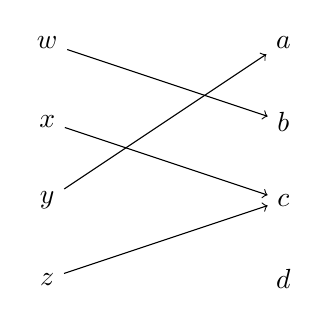
\begin{tikzpicture}
    % domain
    \node (w) at (0, 3) {$w$};
    \node (x) at (0, 2) {$x$};
    \node (y) at (0, 1) {$y$};
    \node (z) at (0, 0) {$z$};
    % co-domain
    \node (a) at (3, 3) {$a$};
    \node (b) at (3, 2) {$b$};
    \node (c) at (3, 1) {$c$};
    \node (d) at (3, 0) {$d$};
    % connections
    \draw[->] (w) -- (b);
    \draw[->] (x) -- (c);
    \draw[->] (y) -- (a);
    \draw[->] (z) -- (c);
  \end{tikzpicture}
  \qquad
  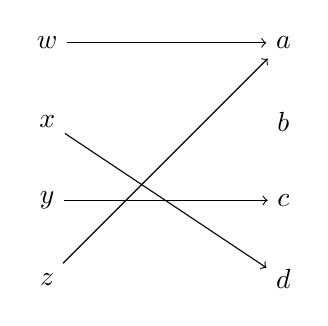
\begin{tikzpicture}
    % domain
    \node (w) at (0, 3) {$w$};
    \node (x) at (0, 2) {$x$};
    \node (y) at (0, 1) {$y$};
    \node (z) at (0, 0) {$z$};
    % co-domain
    \node (a) at (3, 3) {$a$};
    \node (b) at (3, 2) {$b$};
    \node (c) at (3, 1) {$c$};
    \node (d) at (3, 0) {$d$};
    % connections
    \draw[->] (w) -- (a);
    \draw[->] (x) -- (d);
    \draw[->] (y) -- (c);
    \draw[->] (z) -- (a);
  \end{tikzpicture}
\end{center}

\underline{Not} well-defined functions:
\begin{center}
  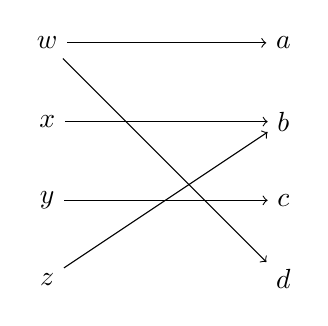
\begin{tikzpicture}
    % domain
    \node (w) at (0, 3) {$w$};
    \node (x) at (0, 2) {$x$};
    \node (y) at (0, 1) {$y$};
    \node (z) at (0, 0) {$z$};
    % co-domain
    \node (a) at (3, 3) {$a$};
    \node (b) at (3, 2) {$b$};
    \node (c) at (3, 1) {$c$};
    \node (d) at (3, 0) {$d$};
    % connections
    \draw[->] (w) -- (a);
    \draw[->] (w) -- (d);
    \draw[->] (x) -- (b);
    \draw[->] (y) -- (c);
    \draw[->] (z) -- (b);
  \end{tikzpicture}
  \qquad
  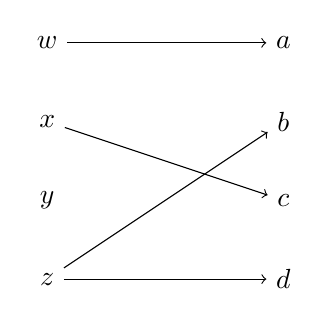
\begin{tikzpicture}
    % domain
    \node (w) at (0, 3) {$w$};
    \node (x) at (0, 2) {$x$};
    \node (y) at (0, 1) {$y$};
    \node (z) at (0, 0) {$z$};
    % co-domain
    \node (a) at (3, 3) {$a$};
    \node (b) at (3, 2) {$b$};
    \node (c) at (3, 1) {$c$};
    \node (d) at (3, 0) {$d$};
    % connections
    \draw[->] (w) -- (a);
    \draw[->] (x) -- (c);
    \draw[->] (z) -- (b);
    \draw[->] (z) -- (d);
  \end{tikzpicture}
\end{center}

For function $f: X \rightarrow Y$, an element $y$ is in the \textbf{range} of $f$
iff there is an $x \in X$ such that $(x, y) \in f$.
\[
  \text{Range of } f = \{y : (x, y) \in f, \text{ for some } x \in X\}
\]
Two functions, $f$ and $g$, are \textbf{equal} if $f$ and $g$ have the same domain and target and
$f(x) = g(x)$ for \underline{every} $x$ in the domain.
\[
  \forall x : f(x) = g(x) \implies f = g
\]

\subsection{Floor and Ceiling functions}
\subsection{Properties of functions}
\subsection{The inverse of a function}
\subsection{Composition of functions}
\subsection{Logarithms and exponents}